\chapter{Organomagnesiumreagentia}\label{ch:b1:organomagnesium}

De meeste nuttige organische moleculen hebben meer koolstofatomen dan
welke goedkope uitgangsstof ook, en het centrale probleem van de synthese
is twee koolstofskeletten te verbinden via een nieuwe C--C-binding. In
een koolstofverbinding is koolstof bijna altijd de elektronenarme partner
van een binding --- met zuurstof, met een halogeen --- en twee
elektronenarme koolstofatomen reageren niet met elkaar. Rond de
eeuwwisseling naar de twintigste eeuw draaide een reagens dat in één kolf
uit een halogeenalkaan en magnesium gemaakt wordt dit om: zijn
koolstofatoom is elektronenrijk, een \omterm{def:b1:electronic-effects:nucleophile}{nucleofiel} dat het koolstofatoom van
een carbonylgroep aanvalt. Daarmee kunnen alcoholen met bijna elk skelet
uit kleinere stukken opgebouwd worden. Dit hoofdstuk toont hoe het
reagens bereid wordt, waarom het een volkomen droge kolf nodig heeft,
waaraan het addeert, en hoe je er een synthese mee plant.

\begin{recall}
\omterm{def:b1:periodicity:electronegativity}{Elektronegativiteit} (\cref{ch:b1:periodicity}); \omterm{def:b1:lewis-resonance-vsepr:lewis-acid}{lewiszuren} en -basen en
de \omterm{def:b1:lewis-resonance-vsepr:lewis-acid}{datieve binding} (\cref{ch:b1:lewis-resonance-vsepr}); \omterm{def:b1:electronic-effects:nucleophile}{nucleofielen},
\omterm{def:b1:electronic-effects:nucleophile}{elektrofielen}, \omterm{def:b1:electronic-effects:curly-arrow}{gebogen pijlen} en de $\mathrm{p}K_a$-schaal van organische
deeltjes (\cref{ch:b1:electronic-effects}); de klasse van een alcohol
(primair, secundair, tertiair) volgt die van zijn koolstofatoom.
\end{recall}

\section{Een grignardreagens bereiden}

\begin{definition}[Organometaalverbinding, grignardreagens]\label{def:b1:organomagnesium:organometallic}
Een \emph{organometaalverbinding}\index{organometaalverbinding} bevat
minstens één koolstof-metaalbinding. Een
\emph{organomagnesiumverbinding}\index{organomagnesiumverbinding} heeft
een C--Mg-binding; het \emph{grignardreagens}\index{grignardreagens}
\ce{RMgX} (X = Cl, Br, I), bereid uit een halogeenalkaan of halogeenareen
en magnesium in een ether, \ce{R-X + Mg -> R-MgX}, is de gangbaarste.
\end{definition}

Het magnesium dringt de C--X-binding binnen. De ether is geen onschuldig
oplosmiddel: magnesium in \ce{RMgX} heeft maar vier \omterm{def:b1:quantum-numbers:configuration}{valentie-elektronen} om
zich heen, en twee ethermoleculen geven het hun \omterm{def:b1:lewis-resonance-vsepr:lewis}{vrije paren}, wat zijn
octet voltooit en het reagens in oplossing houdt.

\begin{omfigure}
\begin{tikzpicture}[font=\small]
  \node (mg) at (0,0) {Mg};
  \node (r) at (-1.5,0) {R};
  \node (x) at (1.5,0) {Br};
  \node (o1) at (0,1.45) {O};
  \node (o2) at (0,-1.45) {O};
  \draw[thick] (r) -- (mg) -- (x);
  \draw[thick, ->, omDef] (o1) -- (mg);
  \draw[thick, ->, omDef] (o2) -- (mg);
  \draw (o1) -- ++(-0.8,0.45) node[left] {\ce{CH3CH2}};
  \draw (o1) -- ++(0.8,0.45) node[right] {\ce{CH2CH3}};
  \draw (o2) -- ++(-0.8,-0.45) node[left] {\ce{CH3CH2}};
  \draw (o2) -- ++(0.8,-0.45) node[right] {\ce{CH2CH3}};
  \node[align=left, anchor=west] at (3.2,0) {twee ethermoleculen geven\\elk een vrij paar (blauw):\\tetraëdrisch magnesium,\\een octet elektronen};
\end{tikzpicture}

{\small Een \omterm{def:b1:organomagnesium:organometallic}{grignardreagens} in ethoxyethaan (diethylether). De \omterm{def:b1:lewis-resonance-vsepr:lewis-acid}{datieve
bindingen} tussen zuurstof en magnesium verklaren waarom het reagens zich
alleen in een ether of een vergelijkbare \omterm{def:b1:lewis-resonance-vsepr:lewis-acid}{lewisbase} vormt.}
\end{omfigure}

\begin{method}[Een grignardreagens bereiden]\label{met:b1:organomagnesium:prepare}
\begin{enumerate}
  \item Droog al het glaswerk in een droogoven; zet een droogbuis met
        calciumchloride op de koeler; gebruik een watervrije ether.
  \item Breng de magnesiumkrullen en een beetje ether in een driehalskolf
        met koeler, druppeltrechter en roerder.
  \item Voeg een kleine portie van het halogenide toe; wanneer de reactie
        op gang komt (troebeling, zacht koken van de ether), voeg dan de
        rest druppelsgewijs toe, met een snelheid die een zachte reflux
        onderhoudt.
  \item Gebruik de oplossing meteen, in dezelfde droge opstelling.
\end{enumerate}
\end{method}

\begin{omfigure}
\begin{tikzpicture}[font=\small]
  \pic at (0,-0.05) {stirrer};
  \pic (f) at (0,0.05) {threeneck={0.35}{omDef!14}};
  \pic at (f-c) {condenser};
  \pic at ($(f-c)+(0,3.2)$) {guardtube};
  \pic[rotate=25] at (f-l) {dropfunnel={0.5}{orange!20}};
  \fill[black!45, rotate around={-25:(f-r)}] ($(f-r)+(-0.17,0)$) rectangle ++(0.34,0.3);
  \draw[->] (2.4,0.9) node[right] {Mg-krullen in droge ether} -- (0.6,0.6);
  \draw[->] (-3.0,3.9) node[left, align=right] {halogenide in ether,\\druppelsgewijs toegevoegd} -- (-1.8,3.4);
  \draw[->] (1.8,5.3) node[right] {koeler (water)} -- (0.45,4.8);
  \draw[->] (1.8,6.6) node[right] {droogbuis met calciumchloride} -- (0.3,6.4);
  \draw[->] (2.4,-0.2) node[right] {magneetroerder} -- (1.3,-0.2);
\end{tikzpicture}

{\small Opstelling voor een grignardreactie: alles wat de lucht kan
bereiken, is gedroogd. De waterdamp van de lucht wordt door de droogbuis
tegengehouden; de koeler stuurt de kokende ether terug naar de kolf.}
\end{omfigure}

\begin{inthelab}[Een reactie die op gang moet komen]
Een grignardbereiding weigert soms op gang te komen: het magnesium is
bedekt met een oxidefilm. Een krul met een glazen staaf fijndrukken, een
\omterm{def:b1:crystals-metals:crystal}{kristal} jood toevoegen of de kolf plaatselijk verwarmen legt vers metaal
bloot. Eenmaal op gang is de reactie exotherm en kookt de ether vanzelf;
de toevoeging wordt dan vertraagd zodat hij niet overkookt. Ethoxyethaan
kookt bij \qty{35}{\celsius} en zijn damp is zeer ontvlambaar: nergens in
het laboratorium een vlam, en een ijsbad binnen handbereik.
% ledger: bp:diethylether
\end{inthelab}


\section{Een sterke base en een nucleofiel}

\begin{definition}[Polariteitsinversie]\label{def:b1:organomagnesium:umpolung}
De \omterm{def:b1:periodicity:electronegativity}{elektronegativiteit} van magnesium (1.31) is veel lager dan die van
koolstof (2.55): in \ce{R-MgX} is de C--Mg-binding gepolariseerd met het
negatieve uiteinde op koolstof, dat zich als een \omterm{def:b1:electronic-effects:intermediates}{carbanion} gedraagt. In
het halogenide \ce{R-X} was hetzelfde koolstofatoom positief (X: 2.96 voor
Br). Een \omterm{def:b1:electronic-effects:nucleophile}{elektrofiel} koolstofatoom omzetten in een \omterm{def:b1:electronic-effects:nucleophile}{nucleofiel} is een
\emph{polariteitsinversie}\index{polariteitsinversie}.
% ledger: en:Mg, en:C, en:Br
\end{definition}


\begin{proposition}[Grignardreagentia worden vernietigd door zure waterstofatomen]\label{prop:b1:organomagnesium:base}
Een \omterm{def:b1:organomagnesium:organometallic}{grignardreagens} reageert \omterm{def:b1:extent-q-and-k:quantitative}{kwantitatief} met water, alcoholen,
carbonzuren, aminen met N--H-bindingen en eindstandige alkynen, waarbij
het alkaan \ce{R-H} ontstaat: \ce{RMgX + H2O -> R-H + Mg(OH)X}.
\end{proposition}

\begin{proof}
Het carbanionachtige koolstofatoom is de base van het koppel
\ce{R-H}/\ce{R^-}, en alkanen zijn verreweg de zwakste zuren van de
organische chemie: van geen enkel proton kan gemeten worden dat het hen
in water verlaat, waar hydroxide de sterkste base is die kan bestaan
(\cref{ch:b1:predominant-reaction}, nivellering). Elk zuur van de lijst
is veel sterker, en de protonoverdracht naar \ce{R^-} heeft een enorme
constante: ze is volledig en snel.
\end{proof}

Dat is de reden voor de droge opstelling: één druppel water vernietigt een
gelijke hoeveelheid reagens. Als voordeel benut plaatst
\ce{CH3CH2MgBr + D2O} een deuteriumatoom precies waar het broom zat.

\section{Addities aan carbonylverbindingen en koolstofdioxide}

Het koolstofatoom van een C=O-groep is \omterm{def:b1:electronic-effects:nucleophile}{elektrofiel}
(\cref{ch:b1:electronic-effects}). Het \omterm{def:b1:organomagnesium:organometallic}{grignardreagens} addeert zijn
R-groep eraan, waarbij het $\pi$-paar van C=O naar zuurstof gaat; een zure
opwerking protoneert daarna het alkoxide.

\begin{omfigure}
\setchemfig{atom sep=2.1em}
\schemestart
\chemfig{@{r}R-[@{rm}]MgBr}
\+
\chemfig{@{cc}C(-[:150]R')(-[:210]R'')=[@{co}]@{o}O}
\arrow{->}
\chemfig{C(-[:150]R')(-[:210]R'')(-[2]R)-O^{-}}
\chemfig{\phantom{.}}\chemfig{^{+}MgBr}
\arrow{->[\ce{H3O+}]}
\chemfig{C(-[:150]R')(-[:210]R'')(-[2]R)-OH}
\schemestop
\chemmove{\draw[->, thick, shorten <=2pt, shorten >=2pt](rm) .. controls +(70:9mm) and +(180:7mm) .. (cc);
          \draw[->, thick, shorten <=2pt, shorten >=2pt](co) .. controls +(90:6mm) and +(90:6mm) .. (o);}
\par\vspace{6pt}

{\small Additie van een \omterm{def:b1:organomagnesium:organometallic}{grignardreagens} aan een keton (of een aldehyde,
$\mathrm{R''} = \mathrm{H}$): het C--Mg-paar vormt de nieuwe C--C-binding,
terwijl het $\pi$-paar van C=O naar zuurstof gaat; het
magnesiumalkoxide wordt in een afzonderlijke stap door verdund zuur
geprotoneerd.}
\end{omfigure}

\begin{proposition}[Alcoholen uit carbonylverbindingen]\label{prop:b1:organomagnesium:carbonyl-addition}
Na zure opwerking geeft een \omterm{def:b1:organomagnesium:organometallic}{grignardreagens} \ce{RMgX}: met methanal een
primaire alcohol \ce{RCH2OH}; met een ander aldehyde $\mathrm{R'CHO}$ een
secundaire alcohol $\mathrm{RR'CHOH}$; met een keton $\mathrm{R'COR''}$ een
tertiaire alcohol $\mathrm{RR'R''COH}$. De nieuwe C--C-binding verbindt R
met het vroegere carbonylkoolstofatoom.
\end{proposition}

\begin{proof}
Het carbonylkoolstofatoom houdt zijn twee substituenten en krijgt R en
een OH erbij (uit het zuurstofatoom van het alkoxide): methanal brengt
twee H mee, een aldehyde één H en één koolstofgroep, een keton twee
koolstofgroepen. De klasse van de alcohol is het aantal koolstofgroepen
op dat koolstofatoom: één, twee of drie.
\end{proof}

\begin{proposition}[Carbonzuren uit koolstofdioxide]\label{prop:b1:organomagnesium:co2}
Een \omterm{def:b1:organomagnesium:organometallic}{grignardreagens} dat op vast koolstofdioxide gegoten wordt, geeft na
aanzuren het carbonzuur \ce{RCOOH} met één koolstofatoom meer:
\ce{RMgX + CO2 -> RCOOMgX}, daarna \ce{RCOOMgX + H3O+ -> RCOOH + Mg^2+ + X- + H2O}.
\end{proposition}

\begin{proof}
\ce{CO2} is een carbonylverbinding waarvan het koolstofatoom aangevallen
wordt zoals dat van een keton; het gevormde carboxylaat is onder deze
omstandigheden te weinig reactief om een tweede R-groep te adderen (een
negatief geladen carbonyl is een slecht \omterm{def:b1:electronic-effects:nucleophile}{elektrofiel}). Zuur protoneert
het.
\end{proof}

\section{Koolstofskeletten opbouwen}

\begin{method}[Een alcohol plannen]\label{met:b1:organomagnesium:plan-alcohol}
\begin{enumerate}
  \item Zoek het koolstofatoom dat de OH draagt in de beoogde alcohol.
  \item Kies een van zijn koolstofgroepen als R (die komt van het
        \omterm{def:b1:organomagnesium:organometallic}{grignardreagens}, bereid uit \ce{R-Br}); de rest van het molecuul,
        met dat koolstofatoom als C=O, is de carbonylpartner.
  \item Som de mogelijke keuzes op (één per koolstofgroep) en geef de
        voorkeur aan die met eenvoudige, beschikbare reagentia.
  \item Controleer dat geen van beide partners een zuur waterstofatoom of
        een tweede carbonylgroep draagt die ook zou reageren.
\end{enumerate}
\end{method}

\begin{example}[2-Fenylbutaan-2-ol]\label{ex:b1:organomagnesium:plan}
Het koolstofatoom dat de OH draagt, heeft een fenyl-, een methyl- en een
ethylgroep. Drie keuzes: fenylmagnesiumbromide met butaan-2-on;
methylmagnesiumbromide met 1-fenylpropaan-1-on; ethylmagnesiumbromide met
1-fenylethaan-1-on (acetofenon). Alle drie werken; de laatste gebruikt
twee van de gangbaarste reagentia.
\end{example}

\begin{history}[Victor Grignard]
\begin{minipage}[t]{0.2\linewidth}\vspace{0pt}
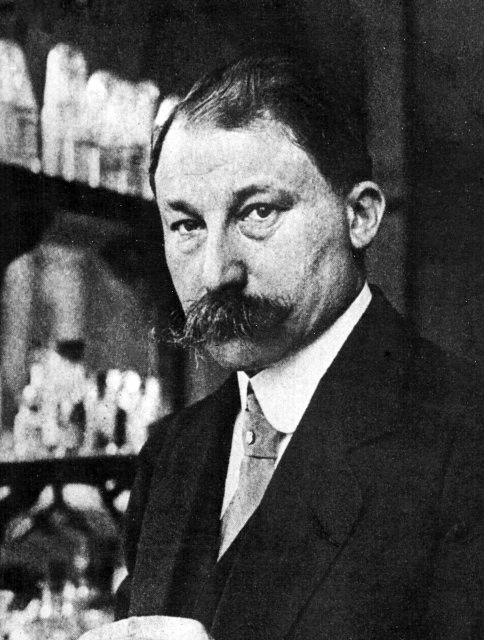
\includegraphics[width=\linewidth]{images/book2/grignard.jpg}
\end{minipage}\hfill
\begin{minipage}[t]{0.76\linewidth}\vspace{0pt}
Het reagens draagt de naam van Victor Grignard, die als promovendus rond
de eeuwwisseling naar de twintigste eeuw ontdekte dat magnesium oplost in
een etheroplossing van een halogeenalkaan en dat de oplossing aan
carbonylverbindingen addeert. Door zijn eenvoud --- één metaal, één
oplosmiddel, één kolf --- werd het de meest gebruikte reactie om
koolstof-koolstofbindingen te vormen van de eeuw, en het leverde zijn
ontdekker een Nobelprijs voor Scheikunde op.
(Foto, publiek domein, Wikimedia Commons.)
\end{minipage}
\end{history}

\section{Oefeningen}

\begin{exercise}[$\star$]\label{exo:b1:organomagnesium:1}
Schrijf de bereiding op van ethylmagnesiumbromide en van
fenylmagnesiumbromide. Geef de polarisatie van de C--Br-binding en van de
C--Mg-binding, met de \omterm{def:b1:periodicity:electronegativity}{elektronegativiteiten}.
\end{exercise}

\begin{exercise}[$\star$]\label{exo:b1:organomagnesium:2}
Wat geeft methylmagnesiumjodide met: water; ethanol; ethaanzuur;
deuteriumoxide \ce{D2O}? Schrijf de reactievergelijkingen op.
\end{exercise}

\begin{exercise}[$\star$]\label{exo:b1:organomagnesium:3}
Geef het product (na zure opwerking) van ethylmagnesiumbromide met
methanal, ethanal, propanon, benzaldehyde en koolstofdioxide. Geef de
klasse van elke alcohol.
\end{exercise}

\begin{exercise}[$\star$]\label{exo:b1:organomagnesium:4}
Waarom mag 4-broombutaan-1-ol niet gebruikt worden om een \omterm{def:b1:organomagnesium:organometallic}{grignardreagens}
te bereiden?
\end{exercise}

\begin{exercise}[$\star\star$]\label{exo:b1:organomagnesium:5}
Schrijf het mechanisme op van de additie van methylmagnesiumbromide aan
ethanal en van de opwerking, met \omterm{def:b1:electronic-effects:curly-arrow}{gebogen pijlen}. Is het product \omterm{def:b1:stereochemistry-in-depth:stereocentre}{chiraal}?
Wordt het als één enkel \omterm{def:b1:stereochemistry-in-depth:enantiomers}{enantiomeer} verkregen? Waarom?
\end{exercise}

\begin{exercise}[$\star\star$]\label{exo:b1:organomagnesium:6}
Stel twee manieren voor om 3-methylpentaan-3-ol te bereiden uit een
\omterm{def:b1:organomagnesium:organometallic}{grignardreagens} en een keton.
\end{exercise}

\begin{exercise}[$\star\star$]\label{exo:b1:organomagnesium:7}
Hoe zou je 2-methylpropaanzuur bereiden uit 2-broompropaan? Bereken de
massa zuur die verkregen wordt uit \qty{12.3}{g} bromide bij een
\omterm{def:b1:extent-q-and-k:fractional-extent}{rendement} van \qty{70}{\percent} ($M$: \ce{C3H7Br} \qty{123.0}{g/mol},
\ce{C4H8O2} \qty{88.0}{g/mol}).
\end{exercise}

\begin{exercise}[$\star\star$]\label{exo:b1:organomagnesium:8}
Een onvoorzichtige student bereidt fenylmagnesiumbromide uit
\qty{0.0500}{mol} broombenzeen in ether die \qty{0.18}{g} water bevat.
Welke fractie van het reagens wordt vernietigd? Welk product ontstaat?
\end{exercise}

\begin{exercise}[$\star\star$]\label{exo:b1:organomagnesium:9}
Bifenyl, \ce{C6H5-C6H5}, is een bijproduct van de bereiding van
fenylmagnesiumbromide. Stel voor hoe het ontstaat, en waarom een trage
toevoeging van broombenzeen aan een overmaat magnesium het beperkt.
\end{exercise}

\begin{exercise}[$\star\star\star$]\label{exo:b1:organomagnesium:10}
Plan twee syntheses van 1-fenylethaan-1-ol uit een \omterm{def:b1:organomagnesium:organometallic}{grignardreagens}, en
een synthese van 2-fenylpropaan-2-ol. Benoem telkens het halogenide dat
het reagens levert.
\end{exercise}

\begin{exercise}[$\star\star\star$]\label{exo:b1:organomagnesium:11}
Leg uit waarom het \omterm{def:b1:organomagnesium:organometallic}{grignardreagens} en de carbonylverbinding gemengd
moeten worden in de volgorde die in het probleem hieronder gekozen is, en
waarom de opwerking gebeurt met koud verdund zuur in plaats van met
alleen water.
\end{exercise}

\begin{exercise}[$\star\star\star$]\label{exo:b1:organomagnesium:12}
Een \omterm{def:b1:organomagnesium:organometallic}{grignardreagens}, gemaakt uit \qty{0.100}{mol} van een bromide, wordt
getitreerd: een deel wordt in een overmaat water gegoten, en het gevormde
basische magnesiumzout wordt getitreerd met zoutzuur: omgerekend naar de
hele oplossing is \qty{0.088}{mol} zuur nodig. Leg het principe uit en
geef het \omterm{def:b1:extent-q-and-k:fractional-extent}{rendement} van de bereiding.
\end{exercise}

\section{Probleem: trifenylmethanol}

\begin{problem}[{Weekendprobleem --- de bereiding van
fenylmagnesiumbromide, de additie ervan aan benzofenon, de opwerking, en
het rendement aan trifenylmethanol}]
\label{pb:b1:organomagnesium:1}
In een droge driehalskolf geven \qty{0.535}{g} magnesium en
\qty{3.14}{g} broombenzeen in watervrij ethoxyethaan
fenylmagnesiumbromide. Daarna wordt druppelsgewijs een oplossing van
\qty{3.28}{g} benzofenon, \ce{(C6H5)2CO}, in dezelfde ether toegevoegd. Na
opwerking met koud verdund zwavelzuur, extractie en herkristallisatie
wordt \qty{3.75}{g} zuiver trifenylmethanol, \ce{(C6H5)3COH}, verkregen,
en wordt \qty{0.15}{g} bifenyl afgescheiden. Molaire massa's
(\unit{g/mol}): Mg 24.3, \ce{C6H5Br} 156.9, \ce{C13H10O} 182.0,
\ce{C19H16O} 260.0, \ce{C12H10} 154.0, \ce{C7H6O2} 122.0.

\medskip
\noindent\textbf{Deel I --- Fenylmagnesiumbromide.}
\begin{enumerate}
  \item Schrijf de reactievergelijking van de bereiding op.
  \item Bereken de hoeveelheden magnesium en broombenzeen. Welke is in
        overmaat?
  \item Waarom moet de opstelling droog zijn? Schrijf de reactie met water
        op.
  \item Wat is de rol van de droogbuis?
  \item Waarom is de ether onmisbaar, naast het oplossen van de
        reagentia?
  \item Bifenyl komt van de reactie van het reagens met broombenzeen.
        Schrijf die op en bereken de hoeveelheid broombenzeen die daardoor
        verloren gaat.
\end{enumerate}

\medskip
\noindent\textbf{Deel II --- De additie.}
\begin{enumerate}[resume]
  \item Bereken de hoeveelheid benzofenon.
  \item Schrijf het mechanisme van de additie op met \omterm{def:b1:electronic-effects:curly-arrow}{gebogen pijlen}.
  \item Welk reagens beperkt de vorming van trifenylmethanol? Houd
        rekening met Deel I.
  \item Is trifenylmethanol \omterm{def:b1:stereochemistry-in-depth:stereocentre}{chiraal}? Verantwoord.
  \item Waarom wordt het benzofenon aan het reagens toegevoegd, en niet
        omgekeerd?
  \item Wat zou een spoor water in de benzofenonoplossing doen?
\end{enumerate}

\medskip
\noindent\textbf{Deel III --- Opwerking.}
\begin{enumerate}[resume]
  \item Schrijf de protonering van het alkoxide op.
  \item Waarom koud verdund zuur gebruiken en niet alleen water?
  \item Waar bevinden trifenylmethanol en de magnesiumzouten zich na
        extractie met ether?
  \item Hoe wordt bifenyl van trifenylmethanol gescheiden? (Bifenyl is
        veel beter oplosbaar in koude petroleumether.)
  \item Welke test bevestigt de zuiverheid van de \omterm{def:b1:crystals-metals:crystal}{kristallen}?
  \item Trifenylmethanol overleeft koud verdund zuur, maar lost op in
        geconcentreerd zwavelzuur tot een diepgeel \omterm{def:b1:electronic-effects:intermediates}{carbokation}. Schrijf de
        vorming ervan op en verklaar zijn stabiliteit (vergelijk met
        \cref{ch:b1:electronic-effects}).
\end{enumerate}

\medskip
\noindent\textbf{Deel IV --- \omterm{def:b1:extent-q-and-k:fractional-extent}{Rendement}, en een ander product.}
\begin{enumerate}[resume]
  \item Bereken de verkregen hoeveelheid trifenylmethanol.
  \item Bereken het \omterm{def:b1:extent-q-and-k:fractional-extent}{rendement} ten opzichte van het beperkende reagens.
  \item Geef twee mogelijke oorzaken van verlies.
  \item Welk product zou ontstaan als het reagens van Deel I (gecorrigeerd
        voor het bifenyl) in plaats daarvan op vast koolstofdioxide
        gegoten was?
  \item Bereken de theoretische massa van dat product.
  \item Schrijf de reactievergelijking van die carboxylering op.
  \item Geef het \omterm{def:b1:extent-q-and-k:fractional-extent}{rendement} aan trifenylmethanol, in procent.
\end{enumerate}
\end{problem}
